
%<<setup-child, include = FALSE>>=
%library(knitr)
%library(ggplot2)
%library(microbenchmark)
%set_parent("../style/preamble.Rnw")
%@

\input{../../2021/style/preamble4tex}
% dependencies: amsmath, amssymb, dsfont
% math spaces
\ifdefined\N
\renewcommand{\N}{\mathds{N}} % N, naturals
\else \newcommand{\N}{\mathds{N}} \fi
\newcommand{\Z}{\mathds{Z}} % Z, integers
\newcommand{\Q}{\mathds{Q}} % Q, rationals
\newcommand{\R}{\mathds{R}} % R, reals
\ifdefined\C
\renewcommand{\C}{\mathds{C}} % C, complex
\else \newcommand{\C}{\mathds{C}} \fi
\newcommand{\continuous}{\mathcal{C}} % C, space of continuous functions
\newcommand{\M}{\mathcal{M}} % machine numbers
\newcommand{\epsm}{\epsilon_m} % maximum error

% counting / finite sets
\newcommand{\setzo}{\{0, 1\}} % set 0, 1
\newcommand{\setmp}{\{-1, +1\}} % set -1, 1
\newcommand{\unitint}{[0, 1]} % unit interval

% basic math stuff
\newcommand{\xt}{\tilde x} % x tilde
\newcommand{\argmin}{\mathop{\mathrm{arg\,min}}} % argmin
\newcommand{\argmax}{\mathop{\mathrm{arg\,max}}} % argmax
\newcommand{\argminlim}{\argmin\limits} % argmin with limits
\newcommand{\argmaxlim}{\argmax\limits} % argmax with limits
\newcommand{\sign}{\operatorname{sign}} % sign, signum
\newcommand{\I}{\mathbb{I}} % I, indicator
\newcommand{\order}{\mathcal{O}} % O, order
\newcommand{\bigO}{\mathcal{O}} % Big-O Landau
\newcommand{\littleo}{{o}} % Little-o Landau
\newcommand{\pd}[2]{\frac{\partial{#1}}{\partial #2}} % partial derivative
\newcommand{\floorlr}[1]{\left\lfloor #1 \right\rfloor} % floor
\newcommand{\ceillr}[1]{\left\lceil #1 \right\rceil} % ceiling
\newcommand{\indep}{\perp \!\!\! \perp} % independence symbol

% sums and products
\newcommand{\sumin}{\sum\limits_{i=1}^n} % summation from i=1 to n
\newcommand{\sumim}{\sum\limits_{i=1}^m} % summation from i=1 to m
\newcommand{\sumjn}{\sum\limits_{j=1}^n} % summation from j=1 to p
\newcommand{\sumjp}{\sum\limits_{j=1}^p} % summation from j=1 to p
\newcommand{\sumik}{\sum\limits_{i=1}^k} % summation from i=1 to k
\newcommand{\sumkg}{\sum\limits_{k=1}^g} % summation from k=1 to g
\newcommand{\sumjg}{\sum\limits_{j=1}^g} % summation from j=1 to g
\newcommand{\summM}{\sum\limits_{m=1}^M} % summation from m=1 to M
\newcommand{\meanin}{\frac{1}{n} \sum\limits_{i=1}^n} % mean from i=1 to n
\newcommand{\meanim}{\frac{1}{m} \sum\limits_{i=1}^m} % mean from i=1 to n
\newcommand{\meankg}{\frac{1}{g} \sum\limits_{k=1}^g} % mean from k=1 to g
\newcommand{\meanmM}{\frac{1}{M} \sum\limits_{m=1}^M} % mean from m=1 to M
\newcommand{\prodin}{\prod\limits_{i=1}^n} % product from i=1 to n
\newcommand{\prodkg}{\prod\limits_{k=1}^g} % product from k=1 to g
\newcommand{\prodjp}{\prod\limits_{j=1}^p} % product from j=1 to p

% linear algebra
\newcommand{\one}{\bm{1}} % 1, unitvector
\newcommand{\zero}{\mathbf{0}} % 0-vector
\newcommand{\id}{\bm{I}} % I, identity
\newcommand{\diag}{\operatorname{diag}} % diag, diagonal
\newcommand{\trace}{\operatorname{tr}} % tr, trace
\newcommand{\spn}{\operatorname{span}} % span
\newcommand{\scp}[2]{\left\langle #1, #2 \right\rangle} % <.,.>, scalarproduct
\newcommand{\mat}[1]{\begin{pmatrix} #1 \end{pmatrix}} % short pmatrix command
\newcommand{\Amat}{\mathbf{A}} % matrix A
\newcommand{\Deltab}{\mathbf{\Delta}} % error term for vectors

% basic probability + stats
\renewcommand{\P}{\mathds{P}} % P, probability
\newcommand{\E}{\mathds{E}} % E, expectation
\newcommand{\var}{\mathsf{Var}} % Var, variance
\newcommand{\cov}{\mathsf{Cov}} % Cov, covariance
\newcommand{\corr}{\mathsf{Corr}} % Corr, correlation
\newcommand{\normal}{\mathcal{N}} % N of the normal distribution
\newcommand{\iid}{\overset{i.i.d}{\sim}} % dist with i.i.d superscript
\newcommand{\distas}[1]{\overset{#1}{\sim}} % ... is distributed as ...


\begin{document}

\lecturechapter{6}{Congruential Generators}
\lecture{CIM1 Statistical Computation}



\begin{vbframe}{Linear congruential generator}

Let $a,c,m \in \N$, then a \textbf{linear congruential generator (LCG)} is defined by
$$
  x_{i+1} = (a x_i + c) \mod m.
$$
Examples:
\begin{itemize}
 \item Marsaglia II: $m = 2^{32}, a = 69069, c = 1$ \\
has maximum possible period of $m$.
\item Longer I: $m = 2^{48}, a = 25214903917, c = 11$ \\
Longer II: $m = 2^{48}, a = 5^{17}, c = 1$ \\
Longer period, specifically designed for 48-bit fraction-arithmetic.
\end{itemize}

% \framebreak
%
% \begin{center}
% \includegraphics{figure_man/lkg.png}
% \end{center}

\end{vbframe}



\begin{vbframe}{Multiplicative congruential generators}

Special case for $c = 0$: \textbf{multiplicative congruential generator (MCG)}

\lz

Let $a, m \in\N$,  we consider the sequence
$$
  x_{i+1} = a x_i \mod m.
$$

\medskip

% Quelle: Monahan (2011), p.281
For example, $x_1, \ldots, x_{m-1}$ is a permutation of the numbers $\{1, \ldots, m-1\}$ if
\begin{itemize}
\item $m$ is a prime,
\item $a^{(m - 1) / q} \mod m \not= 1$ for all prime factors $q$ from $m-1$.
\end{itemize}

\framebreak


\textbf{Example}:

\begin{itemize}
\item $m=17$ (prime number), $a=27$, $x_1 = 5$
% Primfaktor von $16$ ist $2$.\\
% $27^{16/2} \mod 17 = 16 \not= 1$ ist erfüllt.
%
% \lz
%
% Den Seed setzen wir auf eine beliebige Zahl zwischen $1$ und $m-1 = 16$,
% z.B. $x_1 = 5$.
% \begin{eqnarray*}
% x_1 &=& 5 \\[0.2cm]
% x_2 &=& 27 \cdot 5 \mod 17 \\
%     &=& 135 \mod 17 \\
%     &=& (7 \cdot 17 + 16) \mod 17 = 16 \\[0.2cm]
% x_3 &=& 27 \cdot 16 \mod 17 = 7 \\
%     &\hdots&
% \end{eqnarray*}
%
%
% \framebreak

%<<include=FALSE, eval=FALSE>>=
%n = 40L
%m = 17L
%a = 27L
%x = integer(n)
%x[1] = 5L
%for (i in 2:n) {
%  x[i] = (a*x[i-1]) %% m
%}
%x
%library(xtable)
%xtable(matrix(x, byrow = TRUE, ncol = 10L), digits = 0)
%xtable(matrix(x/m, byrow = TRUE, ncol = 10L), digits = 2)
%@

\begin{table}
\begin{footnotesize}
\centering
\begin{tabular}{r|rrrrrrrrrr}
  \hline
i & 1 & 2 & 3 & 4 & 5 & 6 & 7 & 8 & 9 & 10 \\
  \hline
0  & \cellcolor{orange}5 & 16 & 7 & 2 & 3 & 13 & 11 & 8 & 12 & 1 \\
10 & 10 & 15 & 14 & 4 & 6 & 9 & \cellcolor{orange}5 & 16 & 7 & 2 \\
20 & 3 & 13 & 11 & 8 & 12 & 1 & 10 & 15 & 14 &  \ldots \\
\hline
\end{tabular}
\end{footnotesize}
\end{table}

At $i=17$ the sequence starts from the beginning.

%<<include=FALSE, eval=FALSE>>=
%n = 40L
%m = 17L
%a = 26
%x = integer(n)
%x[1] = 5
%for (i in 2:n) {
%  x[i] = (a*x[i-1]) %% m
%}
%x
%library(xtable)
%xtable(matrix(x, byrow = TRUE, ncol = 10L), digits = 0)
%xtable(matrix(x/m, byrow = TRUE, ncol = 10L), digits = 2)
%@

\item  $m=17, a=26$, $x_1 = 5$ \\
$26^{16/2} \mod 17 = 1$

\begin{table}
\begin{footnotesize}
\centering
\begin{tabular}{r|rrrrrrrrrr}
  \hline
i & 1 & 2 & 3 & 4 & 5 & 6 & 7 & 8 & 9 & 10 \\
  \hline
0 & \cellcolor{orange}5 & 11 & 14 & 7 & 12 & 6 & 3 & 10 & \cellcolor{orange}5 & 11 \\
  10 & 14 & 7 & 12 & 6 & 3 & 10 & \cellcolor{orange}5 & 11 & 14 & 7 \\
  20 & 12 & 6 & 3 & 10 & \cellcolor{orange}5 & 11 & 14 & 7 & 12 &  \ldots \\
   \hline
\end{tabular}
\end{footnotesize}
\end{table}

The sequence starts already at $i = 9$ from the beginning, period length $=8$.

\end{itemize}

\framebreak

Concrete implementations:
\begin{itemize}
 \item Very popular for a long time: Lewis Goodman Miller (1969) (e.g., IMSL, early Matlab versions, \ldots):
    $$
      m=2^{31}-1, \qquad a=7^5
    $$
    Reason for choosing $m$: Largest prime number that can be represented as a normal integer on 32-bit machines (period $2^{31} - 2)$.
 \item Infamous (very bad!!!): RANDU
    $$
    m=2^{31}, \qquad a = 65539 = 2^{16}+3
    $$
    Period length of $2^{29}$ and quickly calculated, but major problems with distribution of
    consecutive triplets.
\end{itemize}

\framebreak

For RANDU, the relationship of three consecutive numbers is given by (the following lines are to be understood $\mod 2^{31}$):
\begin{eqnarray*}
x_{i + 1} &=& (2^{16} + 3) x_i \\[0.3cm]
x_{i + 2} &=& (2^{16} + 3)^2 x_i \\
          &=& (2^{32} + 6 \cdot 2^{16} + 9) x_i \footnotemark \\
          &=& (6 \cdot (2^{16} + 3) - 9) x_i \\
          &=& 6 \cdot (2^{16} + 3) x_i - 9 x_i \\
          &=& 6 x_{i + 1} - 9 x_i
\end{eqnarray*}

\footnotetext{$2^{32}$ is a multiple of $m = 2^{31}$, thus canceled out considering $\mod m$.}

\end{vbframe}

\begin{vbframe}{Multiplicative congruential generators}
%<<echo=FALSE>>=
%mkg = function(n, x0 = 1, m = (2^31 - 1), a = (7^5)) {
%  if(x0 < 1) x0 = as.integer(x0 * m)
%  x = integer(n)
%  x[1] = (a * x0) %% m
%  if(n > 1) {
%    for(i in 2:n) {
%      x[i] = (a * x[i-1]) %% m
%    }
%  }
%  x / m
%}
%## Default: Lewis-Goodman-Miller
%@

To illustrate the problem, we use RANDU to generate 12000 random numbers and assign three consecutive numbers to each of the three columns of a matrix.

%<<include = FALSE>>=
%randu = mkg(12000, 1, m = 2^31, a = 2^16 + 3)
%randu3D = as.data.frame(matrix(randu, ncol = 3, byrow = TRUE))
%colnames(randu3D) = c("x1", "x2", "x3")
%@

We are going to visualize the
\emph{points} in a 3D plot.

% <<>>=
% mkg(10, 1)
% x = mkg(600, 1)
% ks.test(x, "punif")
% @

% <<>>=
% par(mfrow = c(1, 3))
% plot(x, type = "l")
% hist(x, freq = FALSE)
% plot(ecdf(x))
% curve(punif, 0, 1, col = 2, add = TRUE)
% @

% <<>>=
% ## Randu
% x = mkg(600, 1, m = 2^31, a = 2^16 + 3)
% ks.test(x, "punif")
% @

% <<>>=
% par(mfrow = c(1, 3))
% plot(x, type = "l")
% hist(x, freq = FALSE)
% plot(ecdf(x))
% curve(punif, 0, 1, col = 2, add = TRUE)
% @

%\framebreak

\vspace*{1cm}

\begin{center}
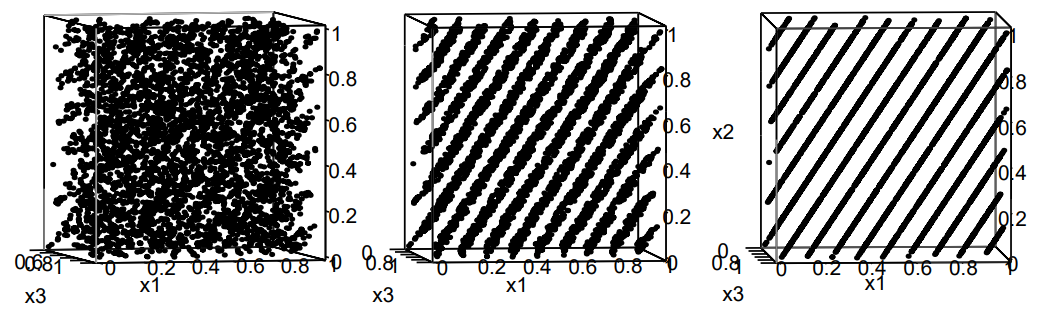
\includegraphics{figure_man/randu.png}
\end{center}

%<<echo=FALSE, rgl=TRUE, include = FALSE>>=
%library(rgl)
%mfrow3d(1, 3)
%with(randu3D, plot3d(x1, x2, x3))
%rgl.viewpoint(theta = -12.8, phi = 3.3, fov = 0, zoom = 0.7, interactive = FALSE)
%with(randu3D, plot3d(x1, x2, x3))
%rgl.viewpoint(theta = -6.8, phi = 3.3, fov = 0, zoom = 0.7, interactive = FALSE)
%with(randu3D, plot3d(x1, x2, x3))
%rgl.viewpoint(theta = -3.8, phi = 3.8, fov = 0, zoom = 0.7, interactive = FALSE)
%@

{\footnotesize \emph{Note:} It is the same plot from three different perspectives.}

% <<>>=
% z = with(randu, (6 * x2 - 9 * x1) %% 1)
% head(cbind(z, randu$x3))
% @
\framebreak

Further examples for MCGs:
\begin{itemize}
 \item Park, Miller, Stockmeyer (1993):  $m = 2^{31} - 1, a = 48271$.
 \item Marsaglia I:  $m = 2^{32}, a = 69069$.
 \item SAS / IMSL:  $m = 2^{31} - 1, a = 397204094$.
 \item Fishman-Moore I, II und III:   $m = 2^{31} - 1$\\
 $a \in \{630360016, 742938285, 950706376 \}$ \\
 (Winner after extensive statistical investigations).
\end{itemize}
\end{vbframe}


\endlecture

\end{document}